\chapter{Grand Unification} 
\section{Running coupling}
The goals of grand unification are
\begin{itemize}
   \item to describe all gauge interactions of the Standard Model via a single simple gauge Group $G_X$ with single coupling $g_X$,
   \item to explain charge quantization.
\end{itemize}

Recall that 
\begin{equation}
  G_\text{SM} = \SU(3)_\text{c} \times \SU(2)_L \times \Uni(1)_Y,
\end{equation}
with three distinct gauge couplings, e.g. running couplings ($\overline{\text{MS}}$) at scale $Q = M_Z \simeq \SI{91}{\giga\eV}$.
\begin{subequations}
   \label{2.2}
\begin{align}
   \alpha_\text{s} (M_Z) &\simeq \num{0.119} \label{2.2a},\\
   \alpha_\text{em}(M_Z) &\simeq 1/128 \label{2.2b},\\
   \sin^2 \theta_W &\simeq \num{0.232} \label{2.2c}.
\end{align}
\end{subequations}

Since $\alpha = g^2 / 4\pi, g_2 = e/ \sin\theta_W, g_Y = e/ \cos\theta_W$,
\begin{subequations}
   \label{2.3}
\begin{align}
   g_3^2 (M_Z) &\simeq \num{1.50} \label{2.3a} \\
   g_2^2 (M_Z) &\simeq \num{0.421} \label{2.3b} \\
   g_Y^2 (M_Z) &\simeq \num{0.128} \label{2.3c}
\end{align}
\end{subequations}
are energy scale dependent, "running" couplings (in $\overline{\text{MS}}$). Dependence on scale $Q$ is given by renormalization group equation (RGE)
\begin{equation}
   \dv{g_i^2 (Q)}{\ln(Q)} = \beta_i (g_k^2)
\end{equation}
To $1$-loop order, $\beta_i$ only depends on $g_i$!

For gauge group $\SU(N)$ ($i \in \{2,3, Y\}$)
\begin{subequations}
   \label{2.5}
\begin{align}
   \feynmandiagram[horizontal=a to b, layered layout, inline=(a.base)]{
      a --[gluon] b --[half left, gluon, edge label=\(v\)] c --[gluon] d,
      b --[half right, gluon] c,
   }; : \quad
   &\beta_i^v = - \frac{g_i^4}{8\pi^2} \cdot C_2(N) \cdot \frac{11}{3} \label{2.5a}\\
   \feynmandiagram[horizontal=a to b, layered layout, inline=(a.base)]{
      a --[gluon] b --[half left, edge label=\(f\)] c --[gluon] d,
      b --[half right] c,
   }; : \quad
   &\beta_i^f = + \frac{g_i^4}{8\pi^2} \cdot T(f) \cdot \frac{2}{3} \label{2.5b}\\
   \feynmandiagram[horizontal=a to b, layered layout, inline=(a.base)]{
      a --[gluon] b --[half left, ghost, edge label=\(s\)] c --[gluon] d,
      b --[half right, ghost] c,
   }; : \quad
   &\beta_i^s = \frac{g_i^4}{8\pi^2} \cdot T(s) \cdot \frac{1}{3} \label{2.5c}
\end{align}
\end{subequations}
with $T = \frac{1}{2}$ for fundamental representation of $\SU(N)$, $C_2(N) = N$ for $\SU(N)$, $C_2(N) = 0$ for $\Uni(1)$, and $T=Y^2$ in $\Uni(1)$. Note that e.g.~in QCD ($\SU(3)$) a quark with three colors forms one single $\SU(3)$ representation (same as $\SU(2)$ doublet)! No need to consider anti-particles, since they are in anti-fundamental representations. The factor $2/3$ accounts for chirality states. Thus
\begin{equation}
   \beta_i = \frac{g_i^4}{8\pi^2} \left[ -\frac{11}{3} C_2(N) + \frac{2}{3} \sum_\text{chiral fermions} T(f) + \frac{1}{3} \sum_\text{complex scalars} T(S) \right]
\end{equation}
In the Standard Model (three generation of fermions, one Higgs doublet)
\begin{align}
      \beta_3 &= \frac{g_3^4}{8\pi^2} \Bigg[ - \frac{11}{3} \cdot 3 + \frac{2}{3} \cdot \frac{1}{2} \cdot 6 \cdot 2 + 0 \Bigg] \notag \\ 
              &=-\frac{g_3^4}{8\pi^2} \cdot 7 \label{2.6}
              \shortintertext{$6$ flavours and $2$ for left- and right-chiral states.}
      \beta_2 &= \frac{g_2^4}{8\pi^2} \left[ -\frac{11}{3} \cdot 2 + \frac{2}{3} \cdot \frac{1}{2} \left( 3 \cdot 3 + 3 \right) + \frac{1}{3} \cdot \frac{1}{2} \cdot 1 \right] \notag \\
              &=-\frac{g_2^4}{8\pi^2} \cdot \frac{19}{6} \label{2.6a}
               \shortintertext{Need to consider color for quark doublets.} \notag
      \beta_Y &= \frac{g_1^4}{8\pi^2} \left\{ 0 + \frac{2}{3} \left[ \left( \frac{1}{6} \right)^2 \cdot 6 \cdot 3 + \left(\frac{2}{3}\right)^2 \cdot 3 \cdot 3 +  \left( -\frac{1}{3} \right)^2 \cdot 3 \cdot 3 + \left(- \frac{1}{2} \right)^2 \cdot 6 + (-1)^2 \cdot 3 \right] + \frac{1}{3} \cdot 2 \cdot \left( \frac{1}{2} \right)^2 \right\} \notag \\ 
              &= \frac{g_Y^4}{8\pi^2} \cdot \frac{41}{6}
              \shortintertext{Count over every fermions considering colors.} \notag
\end{align}


Let
\begin{align}
   \dv{g_1^2}{\ln Q^2} &= - \frac{g^4_i}{8\pi^2} \cdot b_i \notag \\
   \frac{\dd{g_i^2}}{g_i^4} &= - \frac{b_i}{8\pi^2} \dd{\ln Q} \notag \\
   \frac{1}{g_i^2(Q)} &= \frac{1}{g_i^2(M_Z)} + \frac{b_i}{8\pi^2} \ln \frac{Q}{M_Z} \label{2.7}
\end{align}
Straight lines on $\log$ scale for inverse squared gauge couplings. Slopes different for $g_3$ and $g_2$ and they meet at $Q = M_{X^-}$. Equations (\ref{2.7}), (\ref{2.6}), and \eqref{2.6a} give
\begin{equation}
   \ln \frac{M_X}{M_Z} = \left( \frac{1}{g_2^2(M_Z)} - \frac{1}{g_3^2(M_Z)} \right) \cdot \frac{8\pi^2}{b_3 - b_2} \simeq 35 \label{2.8}
\end{equation}
Thus $M_X \simeq \SI{2e17}{\giga\eV}$ and it is beyond reach of conceivable collider. But GUT has measurement consequences.

In running of $g_Y$, only product of $Y\cdot g_Y$ is well-defined. Thus we can test unification of all gauge couplings. Only after normalization of $g_Y$ is fixed. Depends on embedding of hypercharge.
\begin{equation}
   G_{X^-} \stackrel{Q=M_X}{\rightarrow} \SU(3)_\text{c} \times \SU(2) \times \Uni_\text{Y}(1) \stackrel{Q\sim \SI{175}{\giga \eV}}{\rightarrow} \SU(3)_\text{c} \times \Uni(1)_\text{em} \label{2.9}
\end{equation}
For unitarity and renormalizability, the first symmetry breaking should also be due to some Higgs fields!

%%%%%%%%%%%%% Lecture 6
\paragraph{Requirements for $G_{X^-}$} 
\begin{itemize}
   \item must contain $G_\text{SM}$ as subgroup. It must have rank larger than $4$. Rank is the number of diagonal generators. In SM, $2$ from QCD, $1$ from $\SU(2)$ and hypercharge.
   \item must have complex representations, e.g.~$3$ of $\SU(3)$ is complex, $3 \neq \overline{3}$.
\end{itemize}
There is an unique result with rank $4$
\begin{equation*}
   G_{X^-} = \SU(5)
\end{equation*}
(Georgi and Glashow 1974).

\section{$\SU(5)$ Grand Unification}
Recall that $\SU(N)$ has $N^2 - 1$ generators, so $24$ generators for $\SU(5)$. It has rank $=N-1$. Generator can be represented by hermitian $5\times 5$ matrices. Associate first $3$ rows and columns with $\SU(3)$ last $2$ with $\SU(2)$. 

Normalization is as before
\begin{equation}
   \tr(t^a t^b) = \frac{1}{2} \delta^{ab}, \label{2.11}
\end{equation}
with $a,b \in \{1,\dots, 24\}$.

In this representation, the matrices are
\begin{align}
   t^a = \begin{pmatrix} \frac{1}{2} \lambda^a & \pmb{0}_2 \\ \pmb{0}_2 & \pmb{0}_2 \end{pmatrix}
   \shortintertext{with $a=1,\dots,8$ and $\lambda$ are the $\SU(3)$ Gell-Mann matrices.}
   t^{8+i} = \begin{pmatrix} \pmb{0}_3 & \pmb{0}_3 \\ \pmb{0}_3 & \frac{1}{2} \sigma_i \end{pmatrix}
\end{align}
with $i=1,2,3$ and $\sigma^i$ are the $\SU(2)$ Pauli matrices.

Hypercharge generator has to commute with all $\SU(3)$ and $\SU(2)$ generators and it should be traceless. The choice is unique up to overall sign
\begin{equation}
   t^{12} = \frac{1}{2\sqrt{15}} \diag(+2, +2, +2, -3, -3)
\end{equation}

The remaining $12$ generators couple to both $\SU(3)$ and $\SU(2)$
\begin{equation}
   t^{13} = \frac{1}{2} \begin{pmatrix} \pmb{0}_{3\times 3} & A^{13} \\ B & \pmb{0}_{2\times 2}\end{pmatrix}
\end{equation}
with 
\begin{align}
   A^{13} &= \begin{pmatrix} 1 & 0 \\ 0 & 0 \\ 0 & 0 \\ \end{pmatrix}, \\
   B &= \begin{pmatrix} 1 & 0 & 0 \\ 0 & 0 & 1\end{pmatrix}.
\end{align}

$t^{14}$ to $t^{24}$ have similar form, with
\begin{align}
      & A^{15} = \begin{pmatrix} 0 & 0 \\ 1 & 0 \\ 0 & 0 \end{pmatrix}  \quad
      && A^{16} = \begin{pmatrix} 0 & 0 \\ i & 0 \\ 0 & 0 \end{pmatrix}  \quad
      &&& A^{17} = \begin{pmatrix} 0 & 0 \\ 0 & 0 \\ 1 & 0 \end{pmatrix}  \quad
      &&&& A^{18} = \begin{pmatrix} 0 & 0 \\ 0 & 0 \\ i & 0 \end{pmatrix}  \quad
      &&&&& A^{19} = \begin{pmatrix} 0 & 1 \\ 0 & 0 \\ 0 & 0 \end{pmatrix};  \notag \\
      & A^{20} = \begin{pmatrix} 0 & i \\ 0 & 0 \\ 0 & 0 \end{pmatrix}  \quad
      && A^{21} = \begin{pmatrix} 0 & 0 \\ 0 & 1 \\ 0 & 0 \end{pmatrix}  \quad
      &&& A^{22} = \begin{pmatrix} 0 & 0 \\ 0 & i \\ 0 & 0 \end{pmatrix}  \quad
      &&&& A^{23} = \begin{pmatrix} 0 & 0 \\ 0 & 0 \\ 0 & 1 \end{pmatrix}  \quad
      &&&&& A^{24} = \begin{pmatrix} 0 & 0 \\ 0 & 0 \\ 0 & i \end{pmatrix}.  \label{2.12}
\end{align}

\paragraph{Group theory} Decomposition of $\underline{24}$ under $\SU(3) \times \SU(2)$
\begin{equation}
   \underline{24} = (\underline{8}, 1) + (1, 3) + (3,2) + (\overline{3}, 2) + (1,1). \label{2.13}
\end{equation}
The first term corresponds to gluons in $\SU(3)_\text{c}$, second to $W^\pm, W_3$, third and fourth to $X^-$ and $Y$ bosons which are associated with $t^{13}$ to $t^{24}$ and is responsible for $p$-decay, last to hypercharge $B$.

We also need $\SU(5)$ representations for matter and Higgs fields
\begin{align}
   \underline{5} &= (3,1) + (1,\overline{2}) \quad (\text{fundamental rep})  \label{2.14} \\
   \overline{5} &= (\overline{3},1) + (1,2) \quad (\text{anti-fundamental rep}) \quad \label{2.14} \\
   \underline{10} &= (3,2) + (\overline{3}, 1) + (1,1) \quad (\text{anti-symm. rank-}2) \label{2.15}
\end{align}

Writing everything in terms of left-handed fields, we need for one generation of the SM
\begin{align}
   \underbrace{(3,2)}_{q_L} + \underbrace{(\overline{3}, 1)}_{u_R^c} + \underbrace{(\overline{3}, 1)}_{d_R^c} + \underbrace{(1,2)}_{l_L} + \underbrace{(1,1)}_{e_R^c} = \overline{5} + 10. \label{2.16}
\end{align}
In $\SU(2)$, $2 \cong \overline{2}$, since $\sigma_2 \times \overline{l_L}$ transformas like doublet! Minimal coupling of $\overline{5}$ can decide whether $d_R^c$ or $u_R^c$ belongs to $\overline{5}$!
\begin{equation}
   \lag_\text{m.cplg}^{\overline{5}} = \bar{\psi} _{\overline{5}_L} i \slashed{D} \psi_{\overline{5}_L} = \overline{\psi}_{\overline{5}_L} \left( i \slashed{\partial} - g_5 V_\mu^a \gamma^\mu \gamma^\mu t^a \right) \psi_{\overline{5}_L} \label{2.17}
\end{equation}
Write $\overline{5}^T = (q_{R1}^c, q_{R2}^c, q^c_{R 3}, \nu_L, e^-_L)$
\begin{equation}
   \lag_Y^{\overline{5}} = - \frac{g_5}{2\sqrt{15}} B_\mu \left[ + 2 \overline{q^c_R} \gamma^\mu q_R^c - 3 \left( \overline{\nu}_L \gamma^\mu \nu_L + \overline{e^-_L} \gamma^\mu e^-_L \right) \right]. \label{2.18}
\end{equation}
It means
\begin{align}
   Y(q_R^c) = - \frac{2}{3} Y(\nu_L) = + \frac{1}{3}, \label{2.19}
\end{align}
thus $q_R^c = d_R^c$ resides in $\overline{5}$.

$\SU(5)$ also explains charge quantization!
Compare the coupling with SM coupling
\begin{equation*}
   \frac{3 g_5}{2 \sqrt{15}} = \frac{1}{2} g_Y
\end{equation*}
thus
\begin{equation}
   g_Y = \sqrt{\frac{3}{5}} g_5. \label{2.20}
\end{equation}
Holds for exact $\SU(5)$, i.e.~for $Q \geq M_{X^-}$. In SM
\begin{equation}
   \beta(g_Y^2) = \frac{g_Y^4}{8\pi^2} \cdot \frac{41}{6} \Rightarrow b_Y = - \frac{41}{6}
\end{equation}
From (\ref{2.7}) and (\ref{2.8}) and assume all three $g_i$ meet at one point
\begin{align*}
   \frac{1}{g_5^2(M_X)} &= 3.79 \quad \Rightarrow g_5^2(M_X) = 0.264 \\
   \frac{1}{g_Y^2(M_Z)} &= \frac{1}{g_Y^2(M_X)} + \frac{41}{48\pi^2} \ln \frac{M_X}{M_Z} \\
   \Rightarrow & g_Y^2 (M_Z) = 0.107
\end{align*}
This $\SU(5)$ prediction is $\sim 20\%$ off from experimental value $g_Y^2(M_Z) = 0.128$. They are \underline{many} standard deviations apart, but not completely off! Agreement can be improved by adding extra "light" field.

%%%%%%% lecture 7a
(\ref{2.19}) implies that $u^c_R$ must  reside in $\underline{10}$, which can be written as anti-symmetric $5\times 5 $ matrix
\begin{equation}
   \underline{10}_L = \frac{i}{\sqrt{2}} 
   \begin{pmatrix} 
   0 & u_3^c & -u_2^c & -u_1 & -d_1 \\ 
   -u_3^c & 0 & u^c_1 & -u_2 & -d_2 \\
   u_2^c & -u_1^c & 0 & -u_3 & -d_3 \\
   u_1 & u_2 & u_3 & 0 & -e^c \\
   d_1 & d_2 & d_3 & e^c & 0
\end{pmatrix} _L \label{2.22}
\end{equation}
Again the index denotes the colour and the $1/\sqrt{2}$ factor arises because every field appears twice. Note that $L$ for left chiral symbol is "outside", i.e.~$(u^c)_L = u_R^c$.

Gauge i.a.~and kinetic term of $\underline{10}$ cane be found by writing it as an anti-symmetric product $5\times 5 = 10 + 15$ with $10$ being anti-symmetric and $15$ being symmetric.
\begin{equation}
   \lag_{10} = - \left( \overline{\chi}_{10} \right)_{ik} \left[ i \partial_\mu \delta^i_j - 2 g_5 V^a_\mu (t^a)^i_j \right] \gamma^\mu (\chi_{1 0})^{jk} 
                        = - \tr[\overline{\chi}_{10} i \slashed{\partial}\chi_{10} - 2 g_5 \overline{\chi}_{10} V^a_\mu \gamma^\mu t^a \chi_{10}] \label{2.23}
\end{equation}
Coupling is stronger by a factor of 2 (group factor).

\paragraph{Nucleon decay}
The generators $t^{13-24}$ in (\ref{2.17}) and (\ref{2.23}) mediate processes that violate baryon and lepton number!

(\ref{2.17}) contains ($a = 13, \dots, 24$)
\begin{align}
   \lag_{X^-, Y}^{(5)} &= -g_5 \begin{pmatrix} \overline{d^c_R} & \overline{l_L}\end{pmatrix} \begin{pmatrix} 0 & A^a \\ A^{a \dagger} & 0 \end{pmatrix} V_\mu^a \gamma^\mu \begin{pmatrix} d_R^c \\ l_L \end{pmatrix} \notag \\
   &= - g_5 \left[ \overline{l_L}A^{a\dagger} V_\mu^a \gamma^\mu d_R^c + \overline{d^c_R}A^a V_\mu^a \gamma^\mu l_L \right] \notag \\
   &= - \frac{g_5}{\sqrt{2}} \left[ \left( \overline{\nu_L} \overline{Y_\mu} \gamma^\mu + \overline{e^-_L} \overline{X^-_\mu} \gamma^\mu \right)d_R^c + h.c. \right] \label{2.24}
\end{align}
Charge eigenstates $X^-_\mu$ and $Y_\mu$ are associated with $\frac{1}{\sqrt{2}}(V_\mu^{13} \pm i V_\mu^{14}), \dots, \frac{1}{\sqrt{2}}(V_\mu^{23} \pm i V_\mu^{24})$ (see $W_\mu^\pm =\frac{1}{\sqrt{2}} (W_{1\mu} \pm i W_{2\mu})$). $Y$ bosons have electric charge $+\frac{1}{3}$, $X^{-}$ have $+ \frac{4}{3}$. 
\begin{equation}
   Q(X^-) = \frac{4}{3}, \quad Q(Y) = + \frac{1}{3}
\end{equation}
Both are $\SU(3)_\text{c}$ anti-triplets, and member of $\SU(2)$ doublet with $I_3(X^-) = -I_3(Y) = \frac{1}{2}$. From (\ref{2.24}) we would conclude ("leptoquark")
\begin{align}
   B^5(X^-) = B^5(Y) = - \frac{1}{3}  \notag \\
   L^5(X^-) = L^5(Y) = -1 \label{2.25}
\end{align}
($B$ for baryon number and $L$ for lepton number)

From (\ref{2.23})
\begin{equation}
   \lag_{X^-,Y}^{(10)} = g_5 \left[ \overline{X}^\mu \left( \overline{u^c_R} \gamma_\mu u_L + \overline{d_L} \gamma_\mu e^c_R \right) + Y^\mu \left( \overline{u^c_R} \gamma_\mu d_L - \overline{u_L} \gamma_\mu e^c_R \right) \right] + h.c.
\end{equation}
Thus we need 
\begin{align}
   B^{10}(X^-) &= B^{10}(Y)=+\frac{2}{3} \notag \\
   L^{10}(X^-) &= L^{10}(Y) = 0 \label{2.27}
\end{align}

Equations (\ref{2.27}) and (\ref{2.25}) are inconsistent (clash). Thus with $\underline{10}$ present, baryon and lepton numbers are violated!

Note that both assignments give $(B - L) (X^-, Y) = + \frac{2}{3}$. Thus $(B-L)$ is conserved in $\SU(5)$! Still, there is protons decay! E.g. 
\begin{align}
  \begin{tikzpicture}
    \begin{feynman}
       \vertex (i1) {\(u\)};
       \vertex[below=1.5cm of i1] (i2) {\(u\)};
       \vertex[below=0.5cm of i2] (i3) {\(d\)};
       \vertex[below=0.75cm of i1] (h1);
       \vertex[right=1cm of h1] (v1);
       \vertex[right=2cm of v1] (v2);
       \vertex[right=4cm of i1] (f1) {\(e^+\)};
       \vertex[below=1.5cm of f1] (f2) {\(\overline{d}\)};
       \vertex[below=0.5cm of f2] (f3) {\(d\)};
       \diagram*{
          (i1) -- (v1) -- (i2);
          (v1) --[boson, edge label={\(X^-\)}] (v2);
          (f1) -- (v2) -- (f2);
          (i3) -- (f3);
       };
    \end{feynman} 
  \draw [decoration={brace, mirror}, decorate] (i1.north west) -- (i3.south west)
     node [pos=0.5, left] {\(p\)};
  \draw [decoration={brace}, decorate] (f2.north east) -- (f3.south east)
     node [pos=0.5, right] {\(\pi^0\)};
  \end{tikzpicture}
  : p \rightarrow \pi^0 + e^+ \label{2.28}
\end{align}
Rough estimate: Amplitude
\begin{align}
   \mathcal{A} &\sim \frac{g_5^2}{M_{X^-}^2} \cdot m_p^3 \cdot f_\text{hadron} \notag \\
   \tau_p &\sim \SI{1e39}{\year} \cdot \left( \frac{M_X}{\SI{1e17}{\giga\eV}} \right)^4 \label{2.29}
\end{align}
Experimentally $\tau(p\rightarrow e^+\pi^0) \gtrapprox \SI{1e34}{\year}$ (SuperK collaboration). Value (\ref{2.8}) is safe. If $M_X$ is defined as scale where $g_2$ and $\sqrt{\frac{5}{3}}g_Y$ meet, it gives much smaller $M_X$ and there is problem with proton decay! So we need $M_X \gtrapprox \SI{3e15}{\giga\eV}$!

%%%%%%%%%%%%%%%%%%% lecture 7b
\paragraph{Gauge symmetry breaking}
At $Q = M_X$, $\SU(5)$ gets broken into $G_\text{SM} = \SU(3)_\text{c} \times \SU(2)_\text{L} \times \Uni(1)_\text{Y}$ by giving VEV to some Higgs field $\Sigma$. To leave $G_\text{SM}$ unbroken, $\Sigma$ must contain singlet under SM gauge group! The simplest choice would be $\Sigma = \underline{24}$, and it can be written in terms of $t^a$ matrices (\ref{2.12}) as $\SU(5)$ gauge bosons! The desired VEV is
\begin{equation}
   \expval{\Sigma} = v_{X^-} \cdot \frac{1}{2\sqrt{15}} \diag(+2,+2,+2,-3,-3) \label{2.31}
\end{equation}

To get Gauge invariant potential, contract all $\SU(5)$ indices, i.e.~take trace of powers of $\Sigma$! Usually require 
\begin{equation}
   V(\Sigma) =  V(-\Sigma) \label{2.32}
\end{equation}
Thus
\begin{equation}
   V(\Sigma) = \mu^2_{X^-} \tr(\Sigma^2) + \frac{a}{4} \tr(\Sigma^4) + \frac{b}{4} \left( \tr \Sigma^2 \right)^2 \label{2.33}
\end{equation}
Insert (\ref{2.31}) in (\ref{2.33})
\begin{equation*}
   \tr(\expval{\Sigma}^2) = \frac{1}{2} v_X^2, \quad \tr(\expval{\Sigma}^4) = v_X^4 \cdot \frac{7}{120}
\end{equation*}
then
\begin{align}
   V(v_X) &= \frac{1}{2} \mu_X^2 v_x^2 + a v_x^4 \frac{7}{480} + b v_x^4 \frac{1}{16} \label{2.34} \\
   V'(v_X) &= v_x \left[ \mu_X^2 + v_X^2 \left( \frac{7}{120} a + \frac{b}{4} \right)\right]  \stackrel{!}{=} 0 \notag \\
   \mu_X^2 &= - v_X^2 \left( \frac{7a}{120} + \frac{b}{4} \right) < 0
\end{align}
c.f. SM, need negative mass$^2$!

For potential to be bounded from below, i.e.~$V(v_X \rightarrow \infty) > 0$ then $v_X^4 \left( \frac{7a}{480} + \frac{b}{16} \right) > 0$.

Note that other, physically distinct, choice of $\expval{\Sigma}$ are possible, unlike in SM!

\paragraph{Gauge boson masses} from 
\begin{align}
   \lag_\text{g.kin}^\Sigma &= \frac{1}{2} \tr[ \left( D_\mu \Sigma \right)^\dagger \left( D^\mu \Sigma \right)  ] \notag \\
D_\mu \Sigma &= \partial_\mu \Sigma + i g_5 \comm{V_\mu^a t^a}{\Sigma} \label{2.36}
\end{align}
with $\Sigma = t^b \Sigma^b$. The commutator gives term $\sim f^{abc}$. To be compared with gluon self interactions.

Gauge boson mass matrix
\begin{equation}
   M_{V,ab}^2 = - \frac{1}{2} g_5^2 \tr( \comm{t^a}{\expval{\Sigma}} \comm{t^b}{\expval{\Sigma}} )    \label{2.37}
\end{equation}
Gauge bosons $V_\mu^a$ with $\comm{t^a}{\expval{\Sigma}} = 0$ remain massless. It is manifestly true for $V_\mu^1, \dots, V_\mu^{12}$, i.e.~$G_\text{SM}$ is left unbroken.

But with $a>13$
\begin{align*}
   &\begin{pmatrix} 0 & A \\ A^\dagger & 0\end{pmatrix} 
   \begin{pmatrix} 2 & 0 \\ 0 & -3 \end{pmatrix} 
   -
   \begin{pmatrix} 2 & 0 \\ 0 & -3\end{pmatrix}
   \begin{pmatrix} 0 & A \\ A^\dagger & 0 \end{pmatrix}  \\
   &= \begin{pmatrix} 0 & -3A \\ 2A^\dagger & 0\end{pmatrix} 
   - 
   \begin{pmatrix} 0 & 2A \\ -3A^\dagger & 0 \end{pmatrix} \\
   &= 5 \begin{pmatrix} 0 & -A \\ A^\dagger & 0 \end{pmatrix}
\end{align*}
Thus
\begin{align}
   M^2_{V, ab} &= -\frac{1}{2} g_5^2 \cdot \frac{v_X^2}{60} \cdot 25 \cdot \tr
   \begin{pmatrix} 0 & -A^a \\ A^{a\dagger} & 0 \end{pmatrix} 
   \begin{pmatrix} 0 & -A^b \\ A^{b\dagger} & 0 \end{pmatrix} \notag \\
   &= - \frac{5g_5^2 v_X^2}{24} \cdot \tr \begin{pmatrix} -A^a A^{b\dagger} & 0 \\ 0 & -A^{a\dagger}A^b \end{pmatrix}    \notag \\
   &= \underbrace{\frac{5g_5^2}{12} v_X^2}_{M^2_{X^-}} \delta^{ab} \label{2.38}
\end{align}
$M_{X^-}$ can be set (roughly) to "the" unification scale! 

\paragraph{SM Higgs}
For electroweak symmetry breaking, and to generate SM fermion masses, need $\SU(2)$ doublet Higgs field $\phi$. Yukawa couplings need to respect $\SU(5)$ symmetry and thus limit the embedding of $\phi$ into $\SU(5)$ multiplets
\begin{align}
   \text{left-handed SM fermions} &= \overline{5} \oplus 10 \notag\\
   \begin{split}
      \overline{5} \times 10 &= 5 + \overline{45} \\
      10 \times 10 &= \overline{5} + 45 + 50 \\
      \overline{5} \times \overline{5} &= \overline{10} + \overline{15}
   \end{split}
   \label{2.39}
\end{align}
$10$, $15$, and $50$ do not contain $\SU(3)_\text{c} \times \Uni(1)_\text{em}$ singlet. They cannot have VEV and thus they do not play role for fermion masses! 

The simplest choice is to introduce (singlet?)
\begin{equation}
   H_5 = (h^1, h^2, h^3, \phi^+, -\phi^0)^T
\end{equation}
This allows Yukawa terms
\begin{equation}
   \lag_\text{Yuk} = \lambda^d \overline{(\psi_{\overline{5}_L})^c_\alpha} \left( \chi_{10_L} \right)^{\alpha\beta} \left( H^\dagger_5 \right)_\beta - \frac{\lambda^u}{4} \epsilon_{\alpha\beta\delta\epsilon} \overline{(\chi_{10_L})^c}^{\alpha\beta} \left( \chi_{10_L} \right)^{\gamma\delta} H_5^\epsilon \label{2.41}
\end{equation}
They look like Majorana mass terms when written in terms of $\SU(5)$ fields, but become Dirac mass terms in SM.

$\lambda^{d,u}$ are matrices in generation space. $\lambda^d \expval{\phi}$ generates masses for down quarks $(\overline{d_R}d_L)$ and charged leptons $(\overline{e^c_L}e^c_R + h.c. = \overline{e_L}e_R + h.c.)$. It predicts 
\begin{equation}
   m_e = m_d, \quad m_\mu = m_s, \quad m_\tau = m_b \label{2.42}
\end{equation}
at scale $Q=M_X$.
Terms $\sim \lambda^u$ only with $\epsilon=5$ give masses, i.e.~$\alpha,\beta,\gamma,\delta \in \{1,\dots, 4\}$. Only up-type quarks get masses, see (\ref{2.22}), no new predictions!

%%%%%%%% Lecture 8

In order to compare (\ref{2.42}) with experiment, we have to use RGE to run down Yukawa couplings to low energies! Thus we need $\beta$-function of Yukawa couplings. Get contributions from gauge and Yukawa interactions
\begin{align*}
   &\text{QCD corr. } \vcenter{\hbox{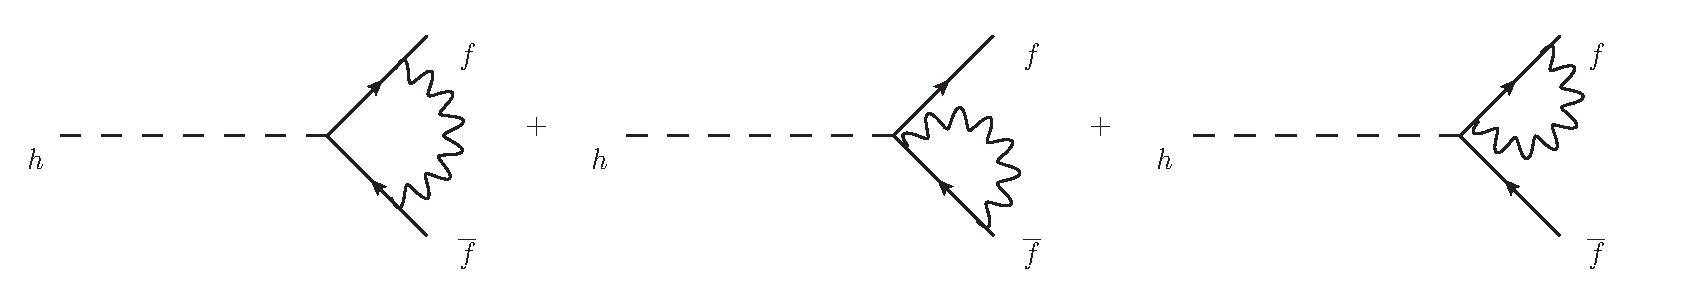
\includegraphics[width=0.7\linewidth]{./figs/yukawa_beta/1.eps}}} \\
   &\SU(2) \times \Uni(1)_\text{Y} \text{ corr. } \vcenter{\hbox{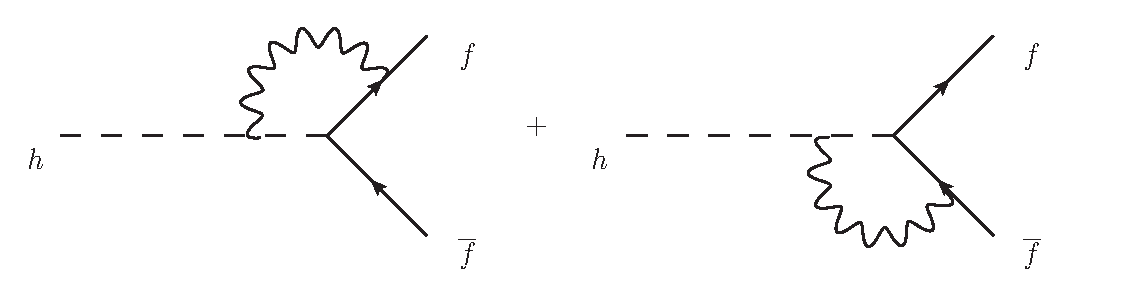
\includegraphics[width=0.5\linewidth]{./figs/yukawa_beta/2.eps}}} \\
   &\text{Yukawa corr. } \vcenter{\hbox{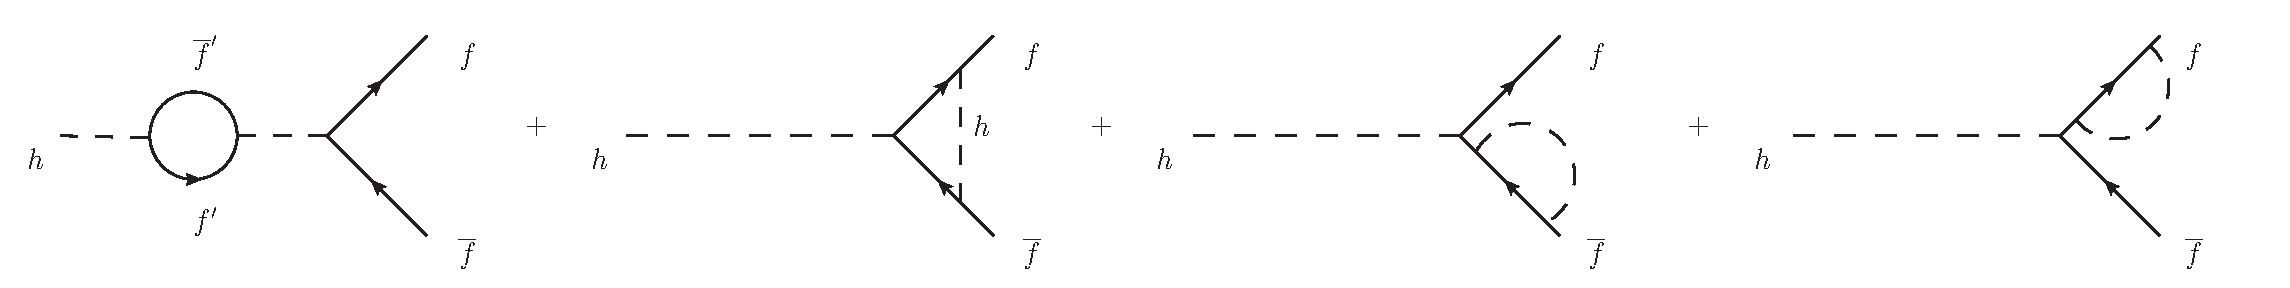
\includegraphics[width=0.95\linewidth]{./figs/yukawa_beta/3.eps}}}
\end{align*}

Couplings to Higgs are ($f=y$)
\begin{align}
   \dv{f_t}{\ln Q} &= \frac{f_t}{16\pi^2} \left[ -3 \left( \frac{8}{3} g_3^2 + \frac{3}{4} g_2^2 + \frac{17}{36} g_Y^2 \right)  + \frac{1}{2} \left( gf_t^2 + 3 f_b^2 + 2f^2_\tau \right) \right] \label{2.43a} \\
   \dv{f_b}{\ln Q} &= \frac{f_b}{16\pi^2} \left[ -3 \left( \frac{8}{3} g_3^2 + \frac{3}{4} g_2^2 + \frac{5}{36}g_Y^2 \right)  + \frac{1}{2} \left( 3 f_t^2 + g f_b^2 + 2f_\tau^2 \right)  \right] \label{2.43b} \\
   \dv{f_\tau}{\ln Q} &=  \frac{f_\tau}{16\pi^2} \left[ -3 \left( \frac{3}{4} g_2^2 + \frac{5}{4} g_Y^2 \right) + \frac{1}{ 2} \left( 6 f_t^2 + 6 f_b^2 + 5 f_\tau^2 \right) \right] \label{2.43c}
\end{align}

They can be solved analytically if Yukawa terms on RHS are neglected
\begin{subequations}
   \label{2.44}
\begin{alignat}{5}
   & f_t(Q) &&= f_t(M_X) \cdot  &&\left[ \frac{\alpha_3 (Q)}{ \alpha_3 (M_X)} \right]^{\frac{4}{b_3}} \cdot &&\left[ \frac{\alpha_2 (Q)}{\alpha_2 (M_X)} \right]^{\frac{g}{8b_2}} \cdot &&\left[ \frac{\alpha_Y (Q)}{\alpha_Y(M_X)} \right]^{\frac{17}{24b_Y}} \label{2.44a}\\
   &f_b(Q) &&= f_b(M_X) \cdot &&\left[ \frac{\alpha_3 (Q)}{\alpha_3 (M_X)} \right]^{\frac{4}{b_3}} \cdot &&\left[ \frac{\alpha_2 (Q)}{\alpha_2(M_X)} \right]^{\frac{g}{8b_2}} \cdot &&\left[ \frac{\alpha_Y (Q)}{\alpha_Y (M_X)} \right]^{\frac{5}{24 b_Y}} \label{2.44b}\\
   &f_\tau (Q) &&= f_\tau (M_X) \cdot &&  && \left[ \frac{\alpha_2(Q)}{\alpha_2(M_X)} \right]^{\frac{g}{8b_2}} \cdot && \left[ \frac{\alpha_Y (Q)}{\alpha_Y(M_X)} \right]^{\frac{15}{8b_Y}} \label{2.44c}
\end{alignat}
\end{subequations}
Details abound the derivation see homework. Note that all three factors in the bracket are larger than $1$. Because $Q < M_x$ and thus $\frac{\alpha_3(Q)}{\alpha_3(M_X)} > 1$ ($4/b_3 > 0$), $\frac{\alpha_2(Q)}{\alpha_2(M_X)} > 1$ ($g/8b_2 > 0$), and $\frac{\alpha_Y(Q)}{\alpha_Y(M_X)} < 1$ ($15/8b_Y < 0$). Thus gauge interactions increase Yukawa couplings when going down in energy!

Yukawa couplings can be ignored when considering ratios of first or second generation fermion masses!
\begin{align}
   \frac{f_s(M_Z)}{f_\mu(M_Z)} &= \frac{f_s(M_X)}{f_\mu (M_X)} \cdot \left[ \frac{\alpha_s(M_Z)}{\alpha_s(M_X)} \right]^{4/7} \cdot \left[ \frac{\alpha_Y(M_Z)}{\alpha_Y(M_X)} \right]^{1/4} \label{2.45}\\
                               &= 1 \cdot 2.7 \cdot 0.9 = 2.4 \label{2.46}
\end{align}
where $f_s(M_X) / f_\mu(M_X) = 1$ in minimal $\SU(5)$. Need $f_s \simeq f_\mu$ at $Q \sim [1,2] \si{\giga\eV}$: (\ref{2.46}) is off by factor $5$. $f_d \simeq 20 f_3$ at $Q \simeq \SI{1}{\giga \eV}$: (\ref{2.46}) is too small by factor $4$.

However, $f_b / f_\tau$ does work more or less! Also $f_t(M_X) < \infty$ gives upper bound on $f_t(m_t)$!

Mixed success of minimal $\SU(5)$. Light fermion masses can be patched up, i.e.~by introducing a Yukawa coupling to $45_H$ or via non-renormalizable operators.

Yukawa interactions (\ref{2.41}) also lead to proton decay through exchange of triplet partner of SM Higgs $h_3$:
\begin{equation}
   \vcenter{\hbox{
         \feynmandiagram[horizontal=v1 to v2]{
            i1[particle=\(d\)] --[fermion] v1 --[anti fermion] i2[particle=\(u\)];
            v1 --[scalar, edge label=\(h_3^*\)] v2;
            f1[particle=\(e\)] --[fermion] v2 --[anti fermion] f2[particle=\(u\)];
         };
   }}: u + d \rightarrow e^+ + \overline{u}
\end{equation}
Need large mass for $h_3$! Simple mass term $m_{H_5}^2 |H_5|^2$ is not sufficient, it would also give positive squared mass $m_{H_5}^2$ to SM Higgs. Then no $\SU(2) \times \Uni(1)_\text{Y}$ breaking!

%%%%% Lecture 9a
We need mass term for $H_5$ that is not $\SU(5)$ invariant. From coupling to $\Sigma$!
\begin{align}
   V(\Sigma, H_5) &= m_H^2 |H_5|^2 + \alpha |H_5|^2 \tr(\Sigma^2) + \beta H_5^\dagger \sigma^2 H_5 \notag \\
                  &\stackrel{\Sigma \rightarrow \expval{\Sigma}}{\longrightarrow} m_H^2 \left( |h|^2 + |\phi|^2 \right) + \alpha \frac{v_x^2}{2} \left( |h|^2 + |\phi|^2 \right) + \beta v_x^2 \left( \frac{1}{15} |h|^2 + \frac{3}{20} |\phi|^2 \right) \label{2.48}
\end{align}
Thus
\begin{align*}
   m_\phi^2 &= m_H^2 + v_x^2 \left( \frac{\alpha}{2} + \frac{3\beta}{20} \right)  \stackrel{!}{=} \order{-M_Z^2}\\
   m_h^2 &= m_H^2 + v_x^2 \left( \frac{\alpha}{2} + \frac{\beta}{15} \right)  \stackrel{!}{=} \order{M_X^2}
\end{align*}
Need $\beta < 0$, and thus delicate cancellation in $m_\phi^2$ to 1 part in $10^{30}$!
\begin{equation}
   m_\phi^2 = m_h^2 + \frac{\beta v_x^2}{12} \stackrel{!}{=} \order{-M_Z^2} \label{2.49}
\end{equation}
From proton decay we must have $m_{h}$ quite large and $v_x$ is roughly the unification scale, but the Higgs mass $m_\phi$ is much lower. This is the \textit{doublet-triplet splitting problem}. Note that even if (\ref{2.49}) is satisfied at tree level, it will be destroyed by loop corrections of order $\frac{\alpha}{\pi} M_X^2$!

Final problem of minimal $\SU(5)$ is there no neutrino masses yet! For renormalizable neutrino masses we need $\nu_R$! Right-handed neutrino is singlet of $\SU(5)$, just added "by hand". If $M_{\nu_R} \sim M_X$, the theory agrees with estimate (\ref{1.61}) in see-saw models roughly. However, in $\SU(5)$, $M_{\nu_R}$ can be anything.

\paragraph{Summary} 

Pro's
\begin{itemize}
   \item explains ordering of gauge couplings
   \item explains quantization of electric charges
   \item get $m_b / m_\tau$ roughly correct (minimal model)
\end{itemize}
Con's
\begin{itemize}
   \item gauge couplings not quite right
   \item if $M_X$ defines via electroweak couplings, protons have too short half life
   \item still need several representations for one generations of SM matter field $10 + \overline{5} (+1)$ ($1$ for right-handed neutrino)
   \item Doublet-triplet splitting requires extreme fine-tuning
\end{itemize}

\section{$\SO(10)$ Unification} 
It solves the third problem!

$\SO(10)$ is the special orthogonal group, rotations in $10$ Euclidean dimensions. Generators are anti-symmetric real $10\times 10$ matrices: $\underline{45}$ is adjoint representation of $\SO(10)$.

$\SO(10)$ has rank $5$, one extra diagonal generator beyond SM.

Decomposition under $\SU(5)$ multiplets
\begin{equation}
   \underline{45} = 24 + 10 + \overline{10} + 1 \label{2.51}
\end{equation}
The extra $\Uni(1)$ generator: gauged $B$-$L$ symmetry!

Whole SM generation fits into $16$-dimensional ("spinor") representation of $\SO(10)$
\begin{equation}
   16  = 10 + \overline{5} + 1 \label{2.51} 
\end{equation}
The $1$ corresponds to $\nu_R$.

SM Higgs fits in fundamental $10$-dimensional representation
\begin{equation}
   10 = 5 + \overline{5} \label{2.52}
\end{equation}
There are two scalar doublets!

Simplest fermion mass term: $16\times 16 \times 10$
\begin{align}
   m_\tau = m_b \quad m_{\nu_R} = m_t \label{2.52}
\end{align}
at unification scale with $m_{\nu}$ Dirac mass. Note that $\nu_R$ is not singlet of $\SO(10)$, then it gets its (large) mass from Higgs mechanism, e.g.~from 126 (1): need to break $B$-$L$. $\SO(10)$ allows several symmetry breaking chains
\begin{equation}
   \SO(10) \stackrel{45}{\longrightarrow} \SU(5) \times \Uni(1)' \stackrel{126}{\longrightarrow} \SU(3) \times \SU(2) \times \Uni(1)_\text{Y} \label{2.53}
\end{equation}
Note that the $\SU(5)$ can be "flipped" $\SU(5)$ with $u^c \in \overline{5}$, $\Uni(1)_\text{Y}$ is combination of $\Uni(1)'$ and $t_{12}$ and $126$ contains $M_{\nu_R}$ generator.

Or
\begin{equation}
   \SO(10) \stackrel{16}{\longrightarrow} \SU(5) \stackrel{45}{\longrightarrow} \SU(3) \times \SU(2) \times \Uni(1)_\text{Y} \label{2.54}
\end{equation}
Or
\begin{equation}
   \SO(10) \stackrel{54}{\longrightarrow} \SU(4) \times \SU(2)_\text{L} \times \SU(2)_\text{R} \stackrel{45}{\longrightarrow} \SU(3) \times \SU(2)_\text{L}\times \SU(2)_\text{R} \times \Uni(1)_\text{B-L} \stackrel{16}{\longrightarrow} \SU(3) \times \SU(2) \times \Uni(1)_\text{Y} \label{2.55}
\end{equation}
(Pati and Salam, 1974). It has intermediate scales, which can be adjusted to obtain exact gauge coupling unification, thus no prediction!

Last step of symmetry breaking might be at relatively low scale, it might have extra gauge gauge bosons, from $\SU(2)_\text{R} \times \Uni(1)_{B-L}$ at accessible energies!

Note that every representation of $\SO(10)$ is anomaly-free! (Not true in $\SU(5)$)

\section{Non-Renormalizable Operators}
GUT scale is not too far from (reduced) Planck scale, $M_p = \SI{2.4e18}{\giga \eV}$ ($G_N = \frac{1}{8\pi M_p^2}$).

Non-Renormalizable operators suppresses by inverse powers of $M_p$ may be important! Such operators are "generically" expected to occur in theories including gravity (supergravity, superstrings), unless forbidden by some symmetry of the full theory.

\paragraph{Example 1} Modification of gauge coupling unification! In renormalizable Yang-Mills theory, the gauge kinetic term
\begin{equation}
   \lag_{\text{g}-\text{k}} = - \frac{1}{4} F^a_{\mu\nu} F^{\mu \nu a} = - \frac{1}{2} \tr (F_{\mu\nu}F^{\mu\nu})  \label{2.56}
\end{equation}
with 
\begin{equation}
   F_{\mu\nu} = \sum_{a} t^a F^a_{\mu\nu}  \label{2.57}
\end{equation}
and $\tr(t^a t^b) = \frac{1}{2} \delta^{ab} $.

In case of $\SU(5)$, from (\ref{2.12})
\begin{equation}
   F_{\mu\nu} = \begin{pmatrix} G_{\mu\nu} + \frac{1}{\sqrt{15}} B_{\mu\nu} \cdot \id_{3} & X^-_{\mu\nu} \\ X^\dagger_{\mu\nu} & W_{\mu\nu} - \frac{3}{2\sqrt{15}}B_{\mu\nu} \id_2  \end{pmatrix} \label{2.58}
\end{equation}
with $G_{\mu\nu}$ gluon field, $X$ gauge field for $X^-$, $Y$ bosons and $W_{\mu\nu}$ for $W$ bosons.


Including a non-renormalizable term, \eqref{2.56} extends to 
\begin{equation}
   \lag_{g-k} = -\frac{1}{2} \tr(F^{\mu\nu}F_{\mu\nu}) - \frac{\kappa}{2M_p} \tr(F_{\mu\nu} \Sigma F^{\mu\nu}) + \order{M_P^{-2}} \label{2.59}
\end{equation}
with $\Sigma$ $\underline{24}$ of $\SU(5)$.

(\ref{2.31}) and (\ref{2.58})
\begin{align*}
   \expval{\Sigma} F_{\mu\nu} &= \frac{v_x}{2\sqrt{15}} \begin{pmatrix} 2 G_{\mu\nu} + \frac{2}{\sqrt{15}}B_{\mu\nu} \id_3 & 2X^-_{\mu\nu} \\ -3X^\dagger_{\mu\nu} & -3 W_{\mu\nu} + \frac{9}{2\sqrt{15}}B_\mu \id_2 \end{pmatrix} \\
   \tr_{\SU(5)}(F_{\mu\nu} \Sigma F^{\mu\nu}) &= \frac{v_x}{2\sqrt{15}} \left[ 2 \tr_{\SU(3)} (G_{\mu\nu}G^{\mu\nu}) - 3 \tr_{\SU(2)} (W_{\mu\nu}W^{\mu\nu}) - \frac{1}{2} B_{\mu\nu} B^{\mu\nu} + \dots  \right]
\end{align*}
(\ref{2.59}) gives for SM gauge bosons
\begin{equation}
   \lag^\text{SM}_{g-k} = -\frac{1}{2} \tr(G_{\mu\nu}G^{\mu\nu}) \left[ 1 + \frac{\kappa v_x}{\sqrt{15} M_p} \right] - \frac{1}{2} \tr(W_{\mu\nu}W^{\mu\nu}) \left[ 1 - \frac{3\kappa v_x}{2\sqrt{15}M_p} \right] - \frac{1}{4} B_{\mu\nu} B^{\mu\nu} \left[ 1 - \frac{\kappa v_x}{\sqrt{15} M_p} \right] + \order{M_p^{-2}} \label{2.60}
\end{equation}

To get standard form of bilinear terms, we have to re-scale fields
\begin{align}
   \begin{split}
      A_\mu^a &\rightarrow \frac{1}{\sqrt{1+ r}} A^a_\mu  \\
      W^i_\mu &\rightarrow \frac{1}{\sqrt{1-3r/2}} W_\mu^i  \\
      B_\mu &\rightarrow \frac{1}{\sqrt{1 - r}} B_\mu  \\
      r &= \frac{\kappa v_x}{\sqrt{15} M_p}
   \end{split}\label{2.61}
\end{align}
In rest of Lagrangian, gauge field always comes multiplied with gauge coupling: (\ref{2.61}) is equivalent to re-scaling of the gauge couplings!
\begin{equation}
   g_3 \rightarrow \frac{1}{\sqrt{1+r}} g_3, \quad g_2 \rightarrow \frac{1}{\sqrt{1-3r/2}} g_2, \quad g_Y \rightarrow \frac{1}{\sqrt{1-r}} g_Y
\end{equation}
This is true at scale $M_X$. After re-scaling, gauge couplings no longer unify! If terms $\order{M_P^{-2}}$are included, we can achieve unification of gauge couplings at any scale of order Planck scale, with any value of GUT gauge coupling!

\paragraph{Example 2} Froggat-Neilsen Mechanism

In order to explain hierarchy of Yukawa couplings, to introduce flavor symmetry. Simplest possibility would be $\Uni(1)_F$.

Flavor symmetry is broken by "flavon" field $f$, which is a singlet under $\SU(5)$.

Introduce small parameter 
\begin{equation}
   \epsilon = \frac{\expval{f}}{M_p} < 1 \label{2.63}
\end{equation}

Assign $U(1)_F$ charges: e.g.
\begin{align}
   \begin{split}
   F(f) &= 1, \\
   F(H_5) &= F(\psi_3) = F(\chi_3) = 0, \\
   F(\psi_2) &= F(\chi_2) = -1, \\
   F(\psi_1) &= F(\chi_1) = -2 \label{2.64}
   \end{split}
\end{align}
with
\begin{align*}
   \psi_3 &= (b^c, \tau, \nu_\tau), 
          &&\chi_3 = (b, t, \tau^c) \\
   \psi_2 &= (s^c, \mu, \nu_\mu ),
          && \chi_2 = (c,s,\mu^c) \\
   \psi_1 &= (d^c, e, \nu_e),
          && \chi_1 = (u, d, e^c)
\end{align*}

Yukawa couplings (\ref{2.41}) only allowed for third generation fermions! More generally:
\begin{equation}
   \lag_\text{Yuk}^\text{eff} = \sum_{i,j} \left[ \lambda_{ij}^d \epsilon^{|F(\psi_1) + F(\chi_j)|}  \overline{\psi^c_i} \chi_j H_5^\dagger -  \frac{\lambda_{ij}^u}{4} \epsilon^{|F(\chi_i)+F(\chi_j)|}\overline{\chi^c_i} \chi_j H_5 + h.c. \right] \label{2.65}
\end{equation}
This can lead to (semi-)realistic quark and lepton mass matrices with all $\lambda^d_{ij}, \lambda^u_{ij} \sim \order{1}$ with 
\begin{equation}
   \epsilon \sim \theta_c \cong \frac{1}{5} \label{2.66}
\end{equation}

We can get structure like (\ref{2.65}) also in a renormalizable theory, by integrating out heavy fermions. E.g.
\begin{align*}
\begin{tikzpicture}   
\begin{feynman}
   \vertex (i) {\(\psi_R\)};
   \vertex[right=2cm of i] (v1);
   \vertex[right=2cm of v1] (v2);
   \vertex[right=2cm of v2] (f) {\(\psi_L\)};
   \vertex[above=2cm of v1] (m1) {\(\expval{f}\)};
   \vertex[above=2cm of v2] (m2) {\(\expval{\phi}\)};
   \diagram*{
      (i) -- (v1) --[insertion=0.5, edge label={\(F_L, F_R\)}] (v2) -- (f),
      (m1) --[scalar] (v1),
      (m2) --[scalar] (v2),
   };
\end{feynman}
\end{tikzpicture}
\end{align*}
gives $\epsilon = \expval{f} / m_F$ suppression.

Symmetry must allow bare $\overline{F_L} F_R$ mass term: $F_{L,R}$ are in vector-like representation of gauge group. Symmetry must allow $\psi_R F_L f$ and $F_R \psi_L \phi$ couplings, but must forbid $\overline{\psi}_R \psi_L H$. Similar to see-saw!
